\documentclass[tikz,border=5pt]{standalone}

\usepackage{amsmath}
\usepackage{fontspec}
\usetikzlibrary{arrows.meta,calc,decorations.pathreplacing,fit,positioning,shadows.blur}

\setmainfont{Arial}

\definecolor{vlblue}{RGB}{44,104,183}
\definecolor{vllight}{RGB}{230,240,255}
\definecolor{robotgreen}{RGB}{53,139,65}
\definecolor{robotlight}{RGB}{232,247,229}
\definecolor{actionorange}{RGB}{230,112,24}
\definecolor{actionlight}{RGB}{255,238,219}
\definecolor{optred}{RGB}{230,0,0}

\begin{document}
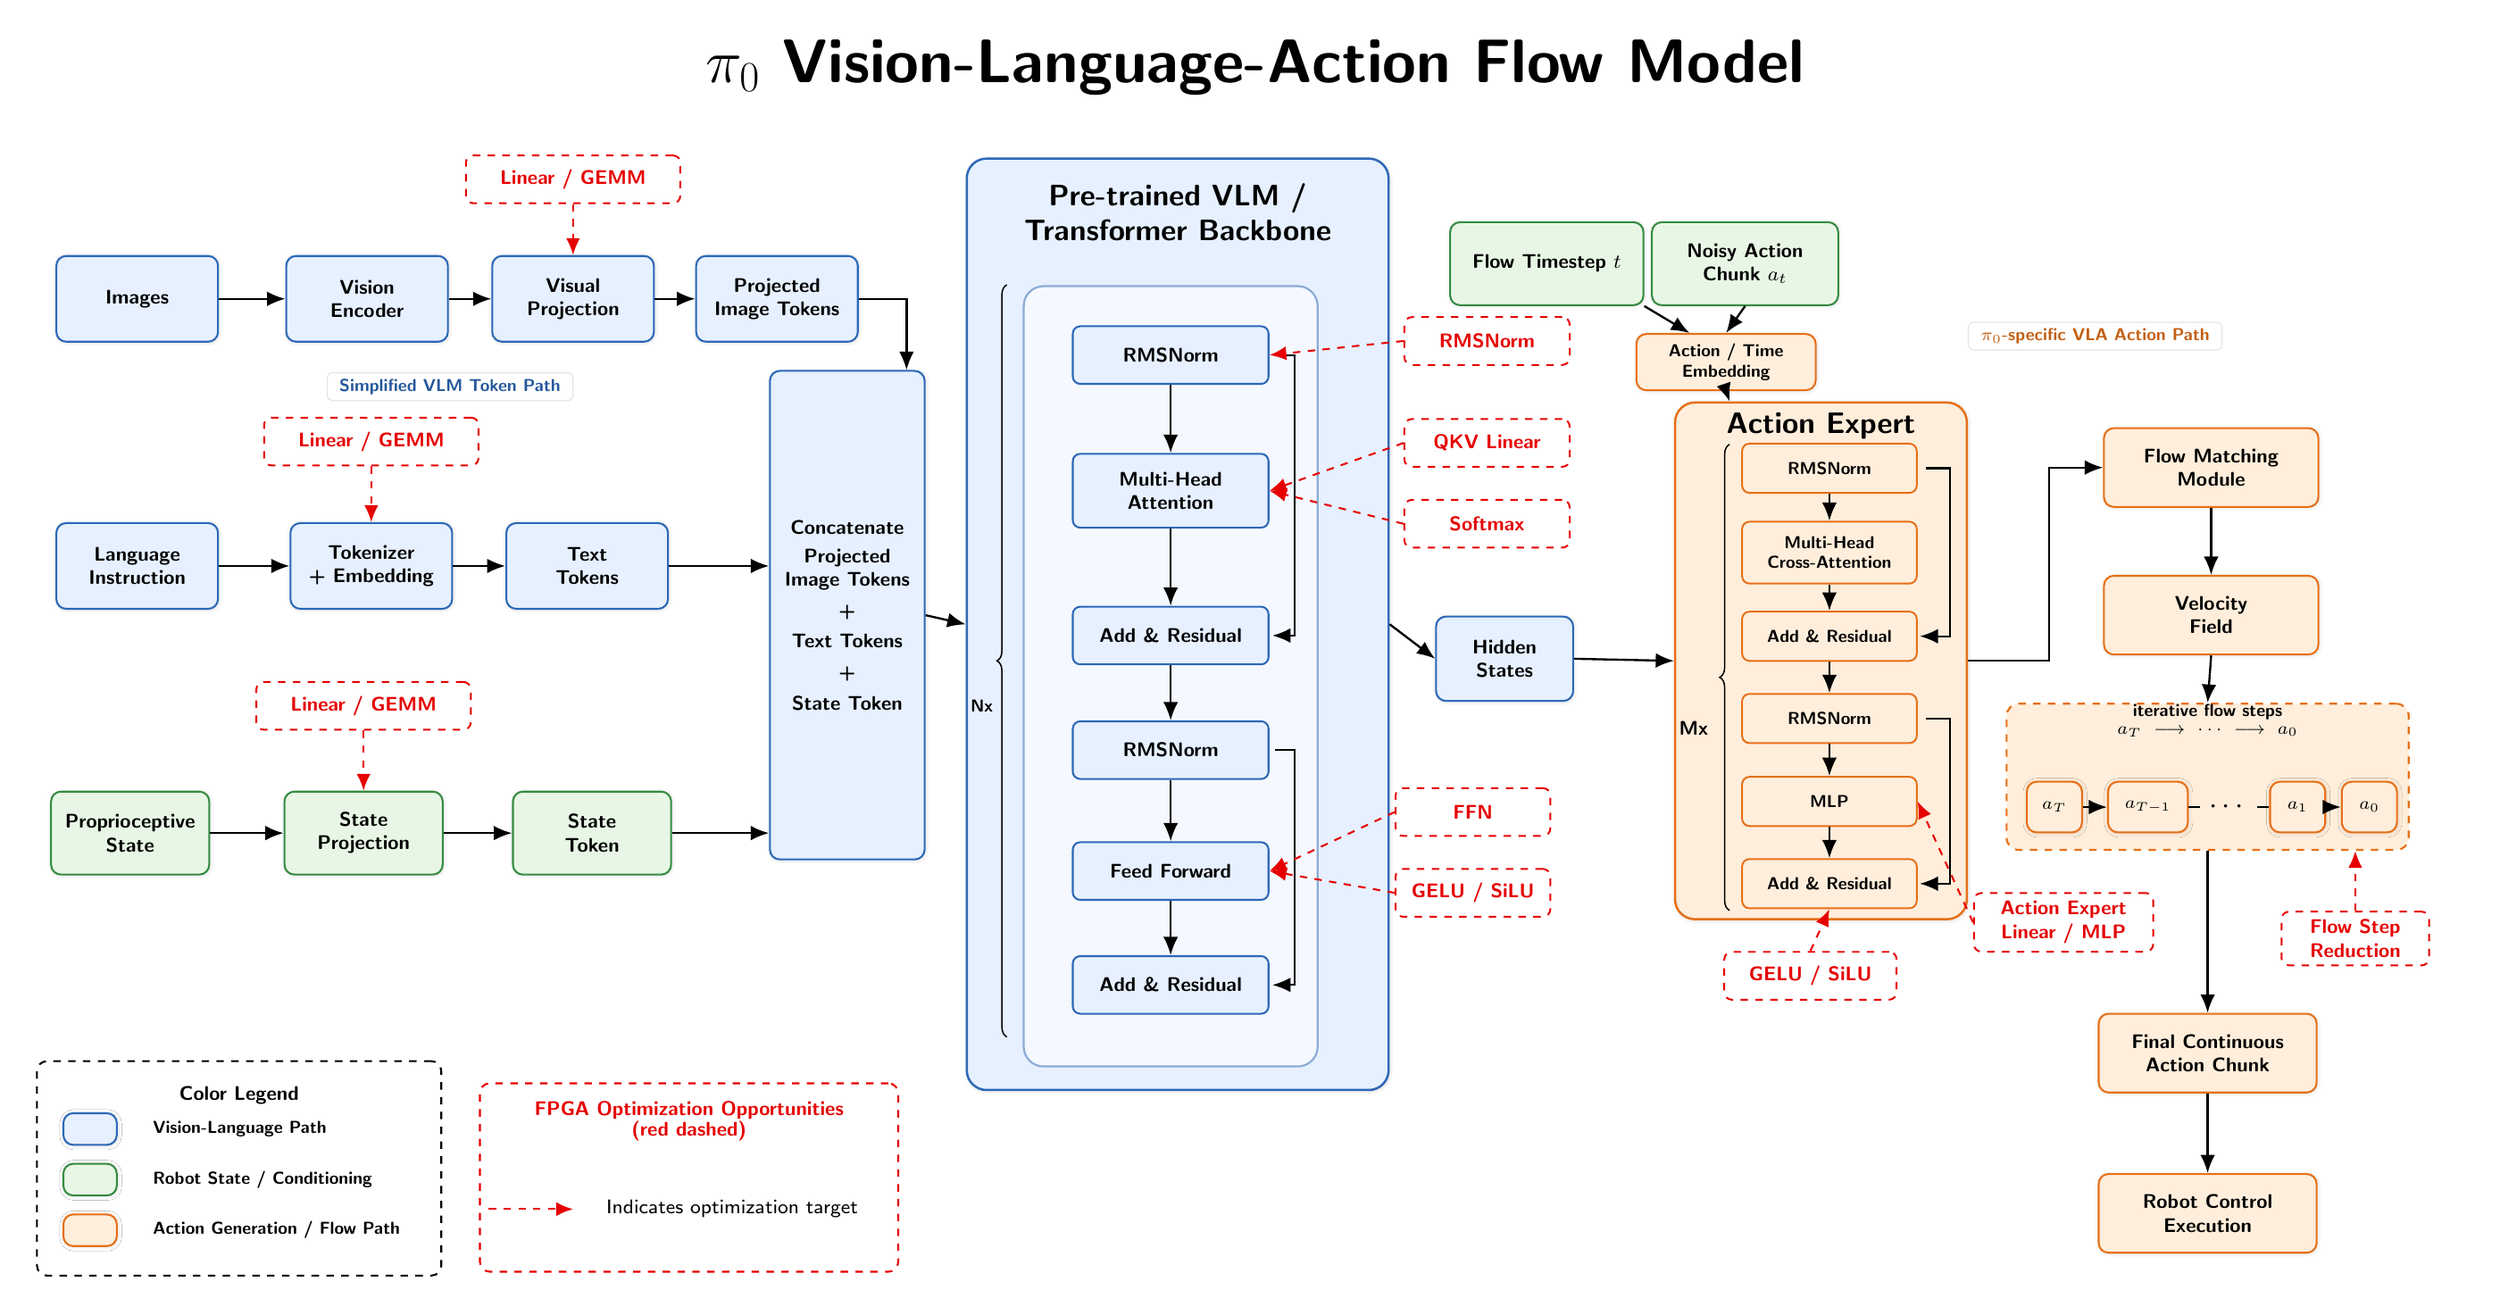
\begin{tikzpicture}[
  x=1cm,y=1cm,
  every node/.style={font=\sffamily},
  flow/.style={-{Latex[length=2.6mm,width=2.1mm]}, line width=0.85pt, draw=black},
  flowclear/.style={-{Latex[length=2.6mm,width=2.1mm]}, line width=0.85pt, draw=black,
    preaction={draw=white,line width=2.5pt}},
  plainline/.style={line width=0.85pt, draw=black},
  repeatbrace/.style={decorate, decoration={brace,amplitude=4.0pt}, line width=0.55pt, draw=black},
  optarrow/.style={-{Latex[length=2.4mm,width=2mm]}, line width=0.75pt, draw=optred, dashed},
  vlbox/.style={
    draw=vlblue, line width=0.75pt, rounded corners=4pt,
    fill=vllight, minimum width=2.3cm, minimum height=1.22cm,
    align=center, text width=2.05cm, font=\sffamily\bfseries\footnotesize,
    blur shadow={shadow blur steps=5,shadow xshift=0.25pt,shadow yshift=-0.25pt,shadow opacity=18}
  },
  greenbox/.style={
    draw=robotgreen, line width=0.75pt, rounded corners=4pt,
    fill=robotlight, minimum width=2.25cm, minimum height=1.18cm,
    align=center, text width=2.0cm, font=\sffamily\bfseries\footnotesize,
    blur shadow={shadow blur steps=5,shadow xshift=0.25pt,shadow yshift=-0.25pt,shadow opacity=16}
  },
  orangebox/.style={
    draw=actionorange, line width=0.75pt, rounded corners=4pt,
    fill=actionlight, minimum width=2.55cm, minimum height=1.12cm,
    align=center, text width=2.28cm, font=\sffamily\bfseries\footnotesize,
    blur shadow={shadow blur steps=5,shadow xshift=0.25pt,shadow yshift=-0.25pt,shadow opacity=16}
  },
  tinyblue/.style={
    draw=vlblue, line width=0.75pt, rounded corners=3pt,
    fill=vllight, minimum width=2.7cm, minimum height=0.82cm,
    align=center, text width=2.55cm, font=\sffamily\bfseries\footnotesize
  },
  tinyorange/.style={
    draw=actionorange, line width=0.72pt, rounded corners=3pt,
    fill=actionlight, minimum width=2.45cm, minimum height=0.70cm,
    align=center, text width=2.25cm, font=\sffamily\bfseries\scriptsize
  },
  callout/.style={
    draw=optred, dashed, line width=0.72pt, rounded corners=3pt,
    fill=white, minimum height=0.68cm, align=center,
    text=optred, font=\sffamily\bfseries\footnotesize
  },
  regionlabel/.style={
    draw=black!10, line width=0.45pt, rounded corners=2pt,
    fill=white, inner xsep=5pt, inner ysep=2.5pt,
    font=\sffamily\bfseries\scriptsize, align=center
  },
  smallmath/.style={font=\sffamily\bfseries\scriptsize},
  labeltext/.style={font=\sffamily\bfseries\footnotesize}
]

\path[use as bounding box] (-0.15,0.05) rectangle (34.7,18.05);

% Title
\node[font=\sffamily\bfseries\fontsize{26}{30}\selectfont] at (17.35,17.45)
  {$\pi_0$ Vision-Language-Action Flow Model};

% Left-side input/tokenization paths
\node[regionlabel, text=vlblue!85!black] at (5.90,12.90) {Simplified VLM Token Path};

\node[vlbox] (images) at (1.45,14.15) {Images};
\node[vlbox] (vision) at (4.72,14.15) {Vision\\Encoder};
\node[vlbox] (vproj) at (7.65,14.15) {Visual\\Projection};
\node[vlbox] (itokens) at (10.55,14.15) {Projected\\Image Tokens};

\node[vlbox] (lang) at (1.45,10.35) {Language\\Instruction};
\node[vlbox] (embed) at (4.78,10.35) {Tokenizer\\+ Embedding};
\node[vlbox] (ttokens) at (7.85,10.35) {Text\\Tokens};

\node[greenbox] (robot) at (1.35,6.55) {Proprioceptive\\State};
\node[greenbox] (sproj) at (4.67,6.55) {State\\Projection};
\node[greenbox] (stoken) at (7.92,6.55) {State\\Token};

\node[vlbox, minimum width=2.2cm, minimum height=6.95cm, text width=1.9cm] (concat) at (11.55,9.65)
  {Concatenate\\[2pt] Projected\\Image Tokens\\[3pt] +\\[3pt] Text Tokens\\[3pt] +\\[3pt] State Token};

\foreach \a/\b in {images/vision,vision/vproj,vproj/itokens,lang/embed,embed/ttokens,robot/sproj,sproj/stoken}
  \draw[flow] (\a.east) -- (\b.west);

\coordinate (imageTokenOut) at ([xshift=0.68cm]itokens.east);
\coordinate (imageTokenIn) at (imageTokenOut |- concat.north);
\draw[flow] (itokens.east) -- (imageTokenOut) -- (imageTokenIn);
\draw[flow] (ttokens.east) -- (concat.west |- ttokens.east);
\draw[flow] (stoken.east) -- (concat.west |- stoken.east);

% FPGA optimization callouts on the left
\node[callout, minimum width=3.05cm] (gemm1) at (7.65,15.85) {Linear / GEMM};
\draw[optarrow] (gemm1.south) -- (vproj.north);

\node[callout, minimum width=3.05cm] (gemm2) at (4.78,12.12) {Linear / GEMM};
\draw[optarrow] (gemm2.south) -- (embed.north);

\node[callout, minimum width=3.05cm] (gemm3) at (4.67,8.36) {Linear / GEMM};
\draw[optarrow] (gemm3.south) -- (sproj.north);

% Pre-trained VLM / Transformer backbone
\node[
  draw=vlblue, line width=0.9pt, rounded corners=8pt, fill=vllight,
  minimum width=6.0cm, minimum height=13.25cm,
  blur shadow={shadow blur steps=6,shadow xshift=0.35pt,shadow yshift=-0.35pt,shadow opacity=18}
] (backbone) at (16.25,9.52) {};

\node[font=\sffamily\bfseries\large, align=center, text width=5.3cm] at (16.25,15.38)
  {Pre-trained VLM /\\ Transformer Backbone};

\node[
  draw=vlblue!55, line width=0.8pt, rounded corners=8pt, fill=white, fill opacity=0.60,
  minimum width=4.18cm, minimum height=11.1cm
] (vlblock) at (16.15,8.78) {};

\node[tinyblue] (rms1) at (16.15,13.35) {RMSNorm};
\node[tinyblue, minimum height=1.05cm] (mha) at (16.15,11.42) {Multi-Head\\Attention};
\node[tinyblue] (add1) at (16.15,9.36) {Add \& Residual};
\node[tinyblue] (rms2) at (16.15,7.73) {RMSNorm};
\node[tinyblue] (ffn) at (16.15,6.01) {Feed Forward};
\node[tinyblue] (add2) at (16.15,4.39) {Add \& Residual};

\draw[flow] (rms1.south) -- (mha.north);
\draw[flow] (mha.south) -- (add1.north);
\draw[flow] (add1.south) -- (rms2.north);
\draw[flow] (rms2.south) -- (ffn.north);
\draw[flow] (ffn.south) -- (add2.north);

\draw[flow] ([xshift=0.08cm]rms1.east) -- ++(0.28,0) |- ([xshift=0.04cm]add1.east);
\draw[flow] ([xshift=0.08cm]rms2.east) -- ++(0.28,0) |- ([xshift=0.04cm]add2.east);
\draw[repeatbrace] (13.82,3.65) -- (13.82,14.35)
  node[pos=0.44,left=2pt,font=\sffamily\bfseries\scriptsize] {Nx};

\draw[flow] (concat.east) -- (backbone.west);

\node[vlbox, minimum width=1.95cm, minimum height=1.20cm, text width=1.55cm] (hidden) at (20.9,9.03)
  {Hidden\\States};
\draw[flow] (backbone.east) -- (hidden.west);

% Transformer FPGA callouts
\node[callout, minimum width=2.35cm] (coRMS) at (20.65,13.55) {RMSNorm};
\draw[optarrow] (coRMS.west) -- (rms1.east);
\node[callout, minimum width=2.35cm] (coQKV) at (20.65,12.10) {QKV Linear};
\draw[optarrow] (coQKV.west) -- (mha.east);
\node[callout, minimum width=2.35cm] (coSoft) at (20.65,10.95) {Softmax};
\draw[optarrow] (coSoft.west) -- (mha.east);
\node[callout, minimum width=2.20cm] (coFFN) at (20.45,6.85) {FFN};
\draw[optarrow] (coFFN.west) -- (ffn.east);
\node[callout, minimum width=2.20cm] (coGeluV) at (20.45,5.70) {GELU / SiLU};
\draw[optarrow] (coGeluV.west) -- (ffn.east);

% Action expert and conditioning
\node[regionlabel, text=actionorange!85!black] at (29.30,13.62)
  {$\pi_0$-specific VLA Action Path};

\node[greenbox, minimum width=2.65cm, text width=2.32cm] (noisy) at (24.32,14.65)
  {Noisy Action\\Chunk $a_t$};

\node[orangebox, minimum width=2.55cm, minimum height=0.80cm, text width=2.25cm,
  font=\sffamily\bfseries\scriptsize] (acttime) at (24.05,13.25)
  {Action / Time\\Embedding};

\node[
  draw=actionorange, line width=0.9pt, rounded corners=8pt, fill=actionlight,
  minimum width=4.15cm, minimum height=7.35cm,
  blur shadow={shadow blur steps=6,shadow xshift=0.35pt,shadow yshift=-0.35pt,shadow opacity=18}
] (expert) at (25.40,9.00) {};
\node[font=\sffamily\bfseries\large, align=center] at (25.40,12.34) {Action Expert};

\node[tinyorange] (ar1) at (25.52,11.74) {RMSNorm};
\node[tinyorange, minimum height=0.88cm] (cross) at (25.52,10.54) {Multi-Head\\Cross-Attention};
\node[tinyorange] (aa1) at (25.52,9.35) {Add \& Residual};
\node[tinyorange] (ar2) at (25.52,8.18) {RMSNorm};
\node[tinyorange] (mlp) at (25.52,7.00) {MLP};
\node[tinyorange] (aa2) at (25.52,5.83) {Add \& Residual};

\draw[flow] (ar1.south) -- (cross.north);
\draw[flow] (cross.south) -- (aa1.north);
\draw[flow] (aa1.south) -- (ar2.north);
\draw[flow] (ar2.south) -- (mlp.north);
\draw[flow] (mlp.south) -- (aa2.north);

\draw[flow] ([xshift=0.12cm]ar1.east) -- ++(0.34,0) |- ([xshift=0.03cm]aa1.east);
\draw[flow] ([xshift=0.12cm]ar2.east) -- ++(0.34,0) |- ([xshift=0.03cm]aa2.east);
\draw[repeatbrace] (24.10,5.45) -- (24.10,12.08)
  node[pos=0.39,left=5pt,font=\sffamily\bfseries\footnotesize] {Mx};

\draw[flow] (noisy.south) -- (acttime.north);
\draw[flow] (acttime.south) -- ([xshift=-1.30cm]expert.north);

\node[greenbox, minimum width=2.75cm, text width=2.40cm] (timestep) at (21.50,14.65)
  {Flow Timestep $t$};
\draw[flow] (timestep.south east) -- ([xshift=-0.52cm]acttime.north);
\draw[flowclear] (hidden.east) -- (expert.west);

\node[callout, minimum width=2.45cm] (coGeluA) at (25.25,4.52) {GELU / SiLU};
\draw[optarrow] (coGeluA.north) -- (aa2.south);
\node[callout, minimum width=2.55cm, text width=2.25cm] (coActionMLP) at (28.85,5.28)
  {Action Expert\\Linear / MLP};
\draw[optarrow] (coActionMLP.west) -- (mlp.east);

% Flow matching path
\node[orangebox, minimum width=3.05cm, text width=2.75cm] (flowmatch) at (30.95,11.75)
  {Flow Matching\\Module};
\node[orangebox, minimum width=3.05cm, text width=2.72cm] (vel) at (30.95,9.65)
  {Velocity\\Field};

\draw[flow] (expert.east) -- ++(1.15,0) |- (flowmatch.west);
\draw[flow] (flowmatch.south) -- (vel.north);

\node[
  draw=actionorange, dashed, line width=0.8pt, rounded corners=5pt,
  fill=actionlight, minimum width=5.72cm, minimum height=2.08cm,
  align=center
] (iter) at (30.90,7.35) {};
\node[font=\sffamily\bfseries\scriptsize, align=center] at (30.90,8.15)
  {iterative flow steps\\[-1pt] $a_T\ \longrightarrow\ \cdots\ \longrightarrow\ a_0$};

\node[orangebox, minimum width=0.72cm, minimum height=0.72cm, text width=0.55cm, font=\sffamily\bfseries\scriptsize] (aT) at (28.72,6.92) {$a_T$};
\node[orangebox, minimum width=1.10cm, minimum height=0.72cm, text width=0.90cm, font=\sffamily\bfseries\scriptsize] (aTm) at (30.05,6.92) {$a_{T-1}$};
\node[font=\sffamily\bfseries\large] (dots) at (31.20,6.92) {$\cdots$};
\node[orangebox, minimum width=0.72cm, minimum height=0.72cm, text width=0.55cm, font=\sffamily\bfseries\scriptsize] (a1) at (32.18,6.92) {$a_1$};
\node[orangebox, minimum width=0.72cm, minimum height=0.72cm, text width=0.55cm, font=\sffamily\bfseries\scriptsize] (a0) at (33.20,6.92) {$a_0$};

\draw[flow] (vel.south) -- (iter.north);
\draw[flow] (aT.east) -- (aTm.west);
\draw[plainline] (aTm.east) -- (dots.west);
\draw[plainline] (dots.east) -- (a1.west);
\draw[flow] (a1.east) -- (a0.west);

\node[callout, minimum width=2.10cm, text width=1.85cm] (stepred) at (33.00,5.05)
  {Flow Step\\Reduction};
\draw[optarrow] (stepred.north) -- ([xshift=2.10cm]iter.south);

\node[orangebox, minimum width=3.10cm, text width=2.78cm] (final) at (30.90,3.42)
  {Final Continuous\\Action Chunk};
\node[orangebox, minimum width=3.10cm, text width=2.78cm] (control) at (30.90,1.14)
  {Robot Control\\Execution};

\draw[flow] (iter.south) -- (final.north);
\draw[flow] (final.south) -- (control.north);

% Legends
\node[
  draw=black, dashed, line width=0.75pt, rounded corners=4pt,
  fill=white, minimum width=5.75cm, minimum height=3.05cm, align=left
] (legend) at (2.90,1.78) {};
\node[font=\sffamily\bfseries\footnotesize] at (2.90,2.82) {Color Legend};
\node[vlbox, minimum width=0.76cm, minimum height=0.45cm, text width=0cm, inner sep=0pt] at (0.78,2.34) {};
\node[anchor=west,font=\sffamily\bfseries\scriptsize] at (1.55,2.34) {Vision-Language Path};
\node[greenbox, minimum width=0.76cm, minimum height=0.45cm, text width=0cm, inner sep=0pt] at (0.78,1.62) {};
\node[anchor=west,font=\sffamily\bfseries\scriptsize] at (1.55,1.62) {Robot State / Conditioning};
\node[orangebox, minimum width=0.76cm, minimum height=0.45cm, text width=0cm, inner sep=0pt] at (0.78,0.90) {};
\node[anchor=west,font=\sffamily\bfseries\scriptsize] at (1.55,0.90) {Action Generation / Flow Path};

\node[
  draw=optred, dashed, line width=0.75pt, rounded corners=4pt,
  fill=white, minimum width=5.95cm, minimum height=2.68cm, align=center
] (optlegend) at (9.30,1.65) {};
\node[text=optred,font=\sffamily\bfseries\footnotesize,align=center] at (9.30,2.45)
  {FPGA Optimization Opportunities\\[-1pt] (red dashed)};
\draw[optarrow] (6.45,1.20) -- (7.65,1.20);
\node[anchor=west,font=\sffamily\footnotesize] at (8.00,1.20) {Indicates optimization target};

\end{tikzpicture}
\end{document}
